\section{Results}
\label{sec:results}

To test the exploration stategy experimentally, we implemented the formulations
and algorithms discussed in Sections~\ref{sec:information_theoretic_objective}-\ref{sec:state_estimation}
in a C++ simulation environment. The simulator assumes a ground robot
constrained to a 2D plane, which is equipped with a noisy laser scanner (range $
= 30$ m, $\sigma = 0.1$ cm), and IMU. Our simulator generates horizontal laser scans
from a meshed point cloud input, and generates IMU observations according to the true
state of the robot. Prior to evaluating CSQMI or building an RRT, we build a map
and localize with respect to it using a custom SLAM implementation that was
developed prior to this project. Our SLAM implementation leverages ICP for laser
odometry~\cite{pomerleau2013comparing}, a histogram filter for
localization~\cite{thrun2005probabilistic}, and a custom 3D mapping framework.

Computing CSQMI requires specification of several parameters. First,

\begin{figure*}
  \centering
  \begin{subfigure}{0.47\textwidth}
    \centering
    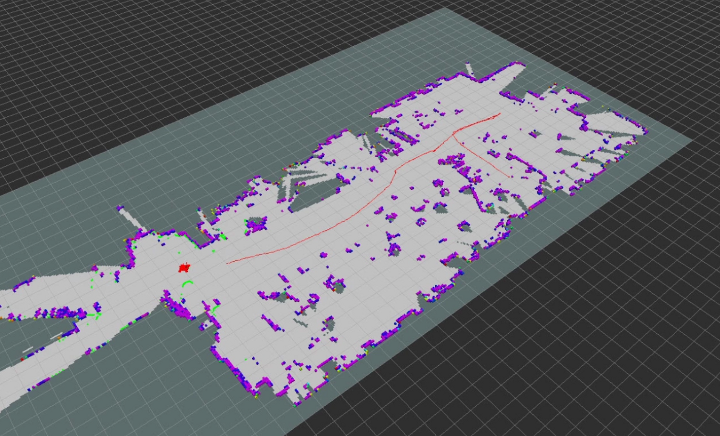
\includegraphics[height=4.3cm]{ground1.png}
    \caption{Map and trajectory\label{fig:ground_bot1}}
  \end{subfigure}
  ~
  \begin{subfigure}{0.47\textwidth}
    \centering
    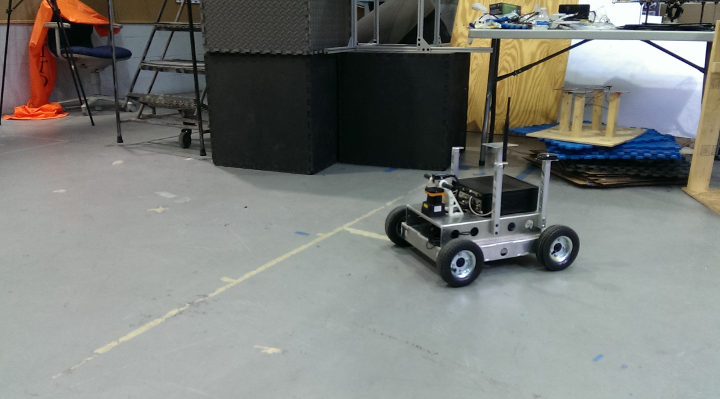
\includegraphics[height=4.3cm]{ground2.png}
    \caption{Ground robot\label{fig:ground_bot2}}
  \end{subfigure}
  \caption{A ground robot mapping while being driven through a cluttered environment.\label{fig:ground_bot}}
\end{figure*}

